%%%% fs-run-mapreduce Optimistic collision management
\label {fs-collision}

We assumed that data items get are flow through the operations in the order. However, this restriction is hard to satisfy, because of asynchrony and possible existence of multiple paths between two nodes. Reordering is of the items does not affect stateless operations: map, flatmap, filter, merge and broadcast, but the stateless one, grouping, depends of the input order.

To handle this problem grouping optimisticaly produce tuples according to the real input order. In case of out-of-order elements we generate the correction tuples.

Therefore, our implementation of grouping need to satisfy following condidion: 

\begin{enumerate}
\item All correct tuples are eventually produced.
\end{enumerate}

The correctness of tuple means that this tuple would be generated if the order assumption was satisfied. 

As it was mentioned, grouping stores all input items in buckets by the value of hash function. Since the order of input items is arbitrary, we can only maintain the order of items within buckets. The next subsections detail how this is satisfied.

\subsubsection{Replaying}

Replaying is used to eventually produce all correct tuples. If the item gets in grouping, according to the meta-information order, nothing is replayed and only the most recent window is produced. If the item is out-of-order, it is inserted in the bucket at the correct location and all tuples, which contain this element, are reproduced. Thereby, replaying guarantees that eventually all correct tuples are generated.

The example of replaying is shown on the figure~\ref{grouping-replaying-figure}. In this example the green item is out-of-order and the window of grouping is 2.

\begin{figure}[htbp]
  \centering
  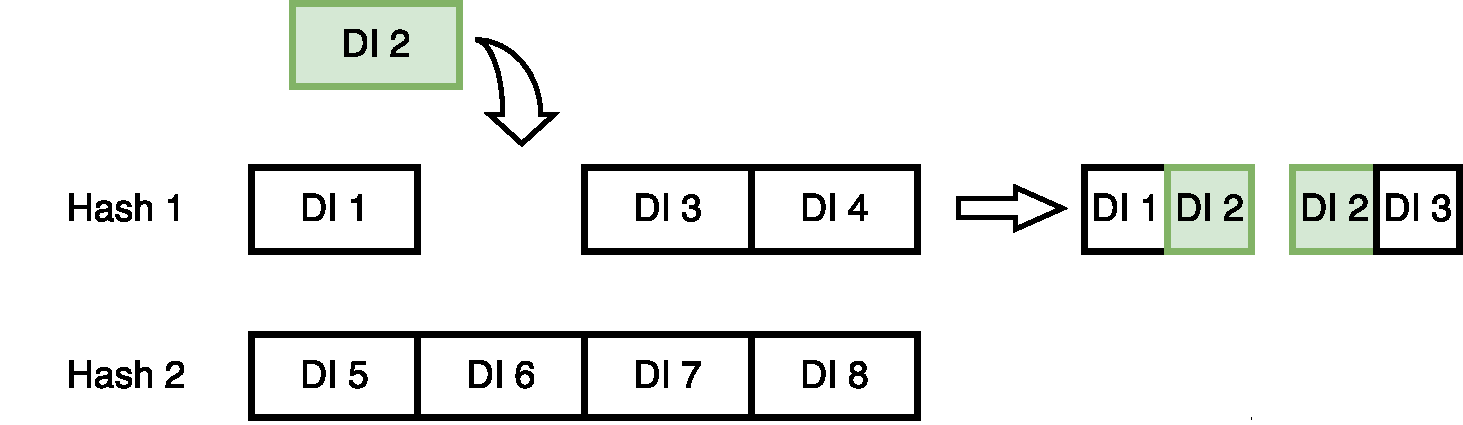
\includegraphics[width=0.48\textwidth]{pics/grouping-replaying}
  \caption{Replaying in grouping}
  \label {grouping-replaying-figure}
\end{figure}
